% Edit this section directly. Styling is in raylo-report.sty.
\section{The credit-risk model and the new champion}
Categorisation is a means to an end: better features for the credit-risk model. The pipeline was run over every transaction for the 49,000 proposals with repayment outcomes, features were rebuilt from the resulting categories, and models were trained on the past and scored on a later window no model had seen. Both out-of-time windows are entirely Plaid, the live provider.

GINI measures how well a score rank-orders bad payers from good, where 0 is random and 1 is perfect. In credit-scoring terms the gaps below are large.

\subsection{From the August model to the champion}
The August report quoted a model capped at 50 features: GINI 0.477 on the three-month outcome and 0.564 on the six-month outcome, against a live model at 0.403 and 0.386. Two things have changed since.

The comparison was tightened. The live model is now refit on the full training window exactly as our models are, which brings its fair figure to 0.382 and 0.385. The as-of filter described in section 6 was applied. The capped model's numbers barely moved, to 0.477 and 0.562.

Then a stricter search was run for a stronger recipe. Where the 50-feature model used 40 individually tracked leaves and rolled the rest up, the champion search gave the model every observed leaf directly. For each of the 275 leaves it built five raw measures per applicant: the number of distinct months the leaf appears in, the transaction count, the debit count, and the debit and credit amounts. That is 1,654 columns once empty ones are dropped, on top of the 304 features already in use. A richer view normalised each by the applicant's totals (share of months, share of transactions, share of spend), reaching 3,150 columns. Eight recipes across XGBoost and LightGBM were compared, varying depth, regularisation, class weighting, a half-weight on Equifax rows and a recency decay that favours recent proposals.

Selection used three rolling validation windows that all sit before the published out-of-time window, and touched that window once, after the recipe was chosen. The final model is a blend of the two tree libraries, averaged over three seeds, with a calibration step so that its probabilities can be read as probabilities.


Out of time, the champion scores 0.533 on the three-month outcome and 0.618 on the six-month one: +0.056 [+0.030, +0.081] and +0.054 [+0.025, +0.084] over the 50-feature model, and +0.138 [+0.097, +0.179] and +0.200 [+0.158, +0.245] over the live model.
This is consistent with section 3: given every column, the taxonomy's detail is worth something to the six-month model, and per-leaf shares and averages are the form in which it is worth most. Persistence remains the dominant feature form (how many distinct months a category appears in matters more than how much was spent), and debt-structure features built from the priority-debt flag remain among the strongest.

\subsection{Holding the champion to 50 features}
The uncapped champion uses between 1,654 and 3,150 input columns, of which 700 to 1,450 carry weight in the fitted trees. That is a different governance proposition from a 50-feature model, where every column can be named, monitored for drift and explained to a reviewer. So the champion recipe was re-run under hard caps of 50, 100 and 200 features, ranking features by their average contribution across both tree libraries and all three seeds on the training window only. Nothing else was re-tuned.

The blend was re-examined at each cap. On the capped folds a single XGBoost matched or beat it on both outcomes, and LightGBM alone fell away at 50 features (0.559 on the six-month outcome). The blend was therefore dropped; the carried-forward model is a single XGBoost, which also keeps the learner identical to the live model's.


\Needspace{200pt}
{\small
\setlength{\TableWidth}{\dimexpr\linewidth-10\tabcolsep\relax}
\begin{longtable}{>{\raggedright\arraybackslash}p{0.34\TableWidth}>{\raggedright\arraybackslash}p{0.1\TableWidth}>{\raggedright\arraybackslash}p{0.15\TableWidth}>{\raggedright\arraybackslash}p{0.15\TableWidth}>{\raggedright\arraybackslash}p{0.26\TableWidth}}
\rowcolor{BlueTint}
\bfseries Champion recipe, scored out of time & \bfseries Features & \bfseries 3-month & \bfseries 6-month & \bfseries 6-month gap to uncapped, 95\% CI \\ \midrule
\endfirsthead
\rowcolor{BlueTint}
\bfseries Champion recipe, scored out of time & \bfseries Features & \bfseries 3-month & \bfseries 6-month & \bfseries 6-month gap to uncapped, 95\% CI \\ \midrule
\endhead
Live model, fair refit &  & 0.382 & 0.385 &  \\ \addlinespace[4pt]
August model, single XGBoost & 50 & 0.477 & 0.562 &  \\ \addlinespace[4pt]
\rowcolor{PeachTint}
Champion recipe, single XGBoost, carried forward & 50 & 0.508 & 0.588 & -0.030 [-0.052, -0.009] \\ \addlinespace[4pt]
Champion recipe, XGBoost + LightGBM blend & 50 & 0.508 & 0.583 & -0.035 [-0.057, -0.014] \\ \addlinespace[4pt]
Champion recipe, blend & 100 & 0.520 & 0.589 & -0.029 [-0.047, -0.010] \\ \addlinespace[4pt]
Champion recipe, blend & 200 & 0.529 & 0.600 & -0.018 [-0.032, -0.004] \\ \addlinespace[4pt]
Champion, uncapped & 1,654 to 3,150 & 0.533 & 0.618 &  \\ \addlinespace[4pt]
\bottomrule
\end{longtable}}
\begin{figure}[H]
\centering
\ChartTitle{Figure 8. Out-of-time GINI: live model, August taxonomy model, and the champion at each feature cap}
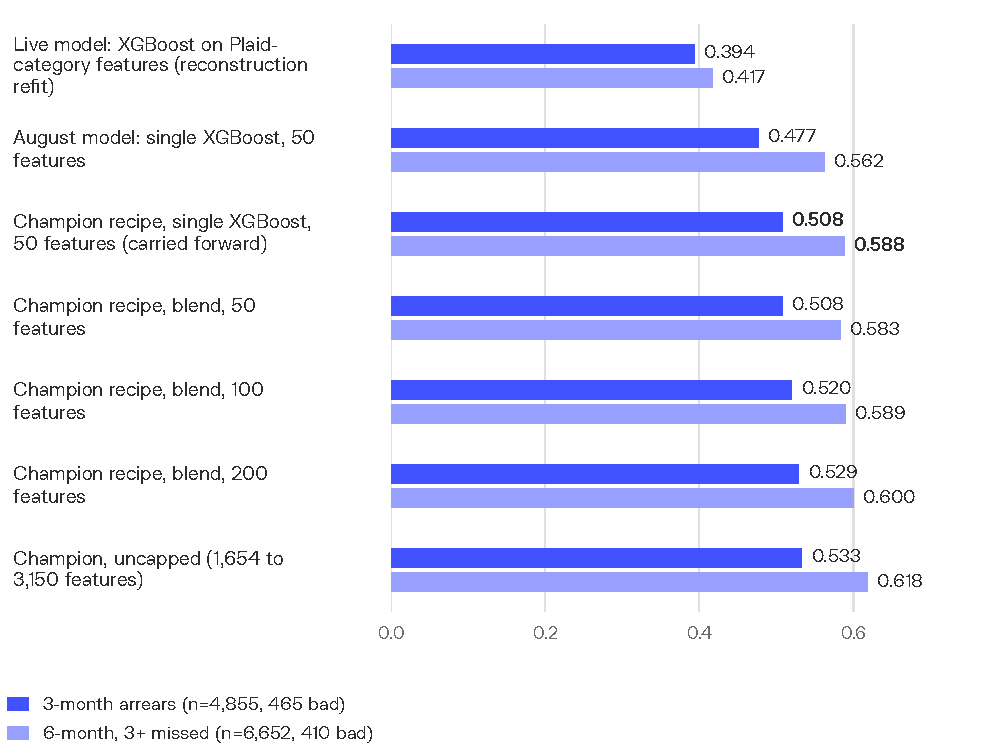
\includegraphics[width=\linewidth]{charts/fig-gini.pdf}
\caption*{Both windows are entirely Plaid. From the 50-feature rows upward the recipe is identical; only the number of columns and the use of a second tree library change.}
\end{figure}
The cap has a real cost and no convenient knee: on the six-month outcome the model is still improving at 200 features. Roughly a third of the champion's gain over the August model is the recipe, which survives a cap, and two thirds is the width, which does not. At 50 features the single-XGBoost recipe beats the August model by +0.031 on the three-month outcome (interval excluding zero) and by +0.024 on the six-month one (interval touching zero).

The 50-feature single-XGBoost champion is carried forward as the reference for the prospective test and for anything that approaches production. Its uplift over the live model, 0.13 GINI on the three-month outcome and 0.20 on the six-month, is what a lending decision would act on, and that barely changes with the cap. The cap gives up the last two to four points in exchange for a model whose every input can be named. The uncapped champion is kept as the ceiling reference; the table above shows what each step of width would buy back.

\begin{tcolorbox}[colback=BlueTint,colframe=Blue,boxrule=0pt,leftrule=2pt,arc=3mm]
Both champions are development recipes. Their out-of-time windows had been used in earlier experiment work, so 0.588 and 0.618 should be read as upper estimates until the prospective test in section 13 is run on a window nobody has touched.
\end{tcolorbox}
